% GNUPLOT: LaTeX picture with Postscript
\begingroup
  \makeatletter
  \providecommand\color[2][]{%
    \GenericError{(gnuplot) \space\space\space\@spaces}{%
      Package color not loaded in conjunction with
      terminal option `colourtext'%
    }{See the gnuplot documentation for explanation.%
    }{Either use 'blacktext' in gnuplot or load the package
      color.sty in LaTeX.}%
    \renewcommand\color[2][]{}%
  }%
  \providecommand\includegraphics[2][]{%
    \GenericError{(gnuplot) \space\space\space\@spaces}{%
      Package graphicx or graphics not loaded%
    }{See the gnuplot documentation for explanation.%
    }{The gnuplot epslatex terminal needs graphicx.sty or graphics.sty.}%
    \renewcommand\includegraphics[2][]{}%
  }%
  \providecommand\rotatebox[2]{#2}%
  \@ifundefined{ifGPcolor}{%
    \newif\ifGPcolor
    \GPcolorfalse
  }{}%
  \@ifundefined{ifGPblacktext}{%
    \newif\ifGPblacktext
    \GPblacktexttrue
  }{}%
  % define a \g@addto@macro without @ in the name:
  \let\gplgaddtomacro\g@addto@macro
  % define empty templates for all commands taking text:
  \gdef\gplbacktext{}%
  \gdef\gplfronttext{}%
  \makeatother
  \ifGPblacktext
    % no textcolor at all
    \def\colorrgb#1{}%
    \def\colorgray#1{}%
  \else
    % gray or color?
    \ifGPcolor
      \def\colorrgb#1{\color[rgb]{#1}}%
      \def\colorgray#1{\color[gray]{#1}}%
      \expandafter\def\csname LTw\endcsname{\color{white}}%
      \expandafter\def\csname LTb\endcsname{\color{black}}%
      \expandafter\def\csname LTa\endcsname{\color{black}}%
      \expandafter\def\csname LT0\endcsname{\color[rgb]{1,0,0}}%
      \expandafter\def\csname LT1\endcsname{\color[rgb]{0,1,0}}%
      \expandafter\def\csname LT2\endcsname{\color[rgb]{0,0,1}}%
      \expandafter\def\csname LT3\endcsname{\color[rgb]{1,0,1}}%
      \expandafter\def\csname LT4\endcsname{\color[rgb]{0,1,1}}%
      \expandafter\def\csname LT5\endcsname{\color[rgb]{1,1,0}}%
      \expandafter\def\csname LT6\endcsname{\color[rgb]{0,0,0}}%
      \expandafter\def\csname LT7\endcsname{\color[rgb]{1,0.3,0}}%
      \expandafter\def\csname LT8\endcsname{\color[rgb]{0.5,0.5,0.5}}%
    \else
      % gray
      \def\colorrgb#1{\color{black}}%
      \def\colorgray#1{\color[gray]{#1}}%
      \expandafter\def\csname LTw\endcsname{\color{white}}%
      \expandafter\def\csname LTb\endcsname{\color{black}}%
      \expandafter\def\csname LTa\endcsname{\color{black}}%
      \expandafter\def\csname LT0\endcsname{\color{black}}%
      \expandafter\def\csname LT1\endcsname{\color{black}}%
      \expandafter\def\csname LT2\endcsname{\color{black}}%
      \expandafter\def\csname LT3\endcsname{\color{black}}%
      \expandafter\def\csname LT4\endcsname{\color{black}}%
      \expandafter\def\csname LT5\endcsname{\color{black}}%
      \expandafter\def\csname LT6\endcsname{\color{black}}%
      \expandafter\def\csname LT7\endcsname{\color{black}}%
      \expandafter\def\csname LT8\endcsname{\color{black}}%
    \fi
  \fi
    \setlength{\unitlength}{0.0500bp}%
    \ifx\gptboxheight\undefined%
      \newlength{\gptboxheight}%
      \newlength{\gptboxwidth}%
      \newsavebox{\gptboxtext}%
    \fi%
    \setlength{\fboxrule}{0.5pt}%
    \setlength{\fboxsep}{1pt}%
    \definecolor{tbcol}{rgb}{1,1,1}%
\begin{picture}(3960.00,1512.00)%
    \gplgaddtomacro\gplbacktext{%
      \csname LTb\endcsname%%
      \put(330,600){\makebox(0,0)[r]{\strut{}\footnotesize$0$}}%
      \csname LTb\endcsname%%
      \put(330,832){\makebox(0,0)[r]{\strut{}\footnotesize$3$}}%
      \csname LTb\endcsname%%
      \put(330,1095){\makebox(0,0)[r]{\strut{}\footnotesize$6$}}%
      \put(130,885){\makebox(0,0)[r]{\strut{}\rotatebox{90}{\footnotesize Frequency}}}%
      \csname LTb\endcsname%%
      \put(330,1360){\makebox(0,0)[r]{\strut{}\footnotesize$9$}}%
      \put(581,300){\makebox(0,0){\strut{}\footnotesize0}}%
      % \put(701,220){\makebox(0,0){\strut{}0.004215}}%
      % \put(820,220){\makebox(0,0){\strut{}0.007025}}%
      % \put(939,220){\makebox(0,0){\strut{}0.009815}}%
      % \put(1058,220){\makebox(0,0){\strut{}0.0126}}%
      % \put(1178,220){\makebox(0,0){\strut{}0.015449999999999998}}%
      % \put(1297,220){\makebox(0,0){\strut{}0.018299999999999997}}%
      \put(1416,300){\makebox(0,0){\strut{}\footnotesize0.02}}%
      % \put(1535,220){\makebox(0,0){\strut{}0.023899999999999998}}%
      % \put(1655,220){\makebox(0,0){\strut{}0.0267}}%
      % \put(1774,220){\makebox(0,0){\strut{}0.0295}}%
      % \put(1893,220){\makebox(0,0){\strut{}0.0323}}%
      % \put(2013,220){\makebox(0,0){\strut{}0.0351}}%
      % \put(2132,220){\makebox(0,0){\strut{}0.0379}}%
      \put(2251,300){\makebox(0,0){\strut{}\footnotesize0.04}}%
      \put(2000,100){\makebox(0,0){\strut{}\footnotesize  Classifier mean best accuracy variance}}
      % \put(2370,220){\makebox(0,0){\strut{}0.04355}}%
      % \put(2490,220){\makebox(0,0){\strut{}0.0464}}%
      % \put(2609,220){\makebox(0,0){\strut{}0.0492}}%
      % \put(2728,220){\makebox(0,0){\strut{}0.052000000000000005}}%
      % \put(2847,220){\makebox(0,0){\strut{}0.0548}}%
      % \put(2967,220){\makebox(0,0){\strut{}0.0576}}%
      \put(3086,300){\makebox(0,0){\strut{}\footnotesize0.06}}%
      % \put(3205,220){\makebox(0,0){\strut{}0.0632}}%
      % \put(3324,220){\makebox(0,0){\strut{}0.066}}%
      % \put(3444,220){\makebox(0,0){\strut{}0.0688}}%
    }%
    \gplgaddtomacro\gplfronttext{%
    }%
    \gplbacktext
    \put(0,-120){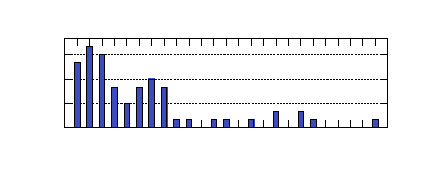
\includegraphics[width={194.00bp},height={90.60bp}]{images/std_accuracy_gamma_losses}}%
    \gplfronttext
  \end{picture}%
\endgroup
